\selectlanguage{ngerman}%
\frenchspacing%
\begin{ledgroupsized}[r]{120mm}%
\footnotesize%
\pstart%
\noindent\textbf{Überlieferung:}%
\pend%
\end{ledgroupsized}%
\begin{ledgroupsized}[r]{114mm}%
\footnotesize%
\pstart%
\parindent -6mm%
\makebox[6mm][l]{\textit{L}}%
Aufzeichnung:
LH~XXXVII,\;3 Bl.\;65.
Ein Blatt 16\textsuperscript{o},
Ränder beschnitten;
\href{\Scan{LH_37_03_065wz}}{Fragment} eines Wasserzeichens:
niedersächsisches Papier. %
Dreiviertel Seite auf Bl.\;65\:r\textsuperscript{o}.
Bl.\;65\:v\textsuperscript{o} überliefert lediglich die \href{\Scan{LH_37_03_065v}}{Reste} eines nicht ermittelten Briefes von fremder Hand: %
\textit{Gestern habe} \textlangle...\textrangle\ \lbrack/\rbrack%
\edlabel{LH_37_03_065_065v_hans-1}
\textit{Meister Hans} \textlangle...\textrangle\ \lbrack/\rbrack%
\edlabel{LH_37_03_065_065v_hans-2}
\textit{so Ew. Herr} \textlangle...\textrangle\ \lbrack/\rbrack\
\textit{gen, uns da}\textlangle...\textrangle\ \lbrack/\rbrack\
\textit{wollen.} \textlangle...\textrangle\ \lbrack/\rbrack\
\textit{In} \textlangle...\textrangle%
\indexN{\textls{Linsen}, Hans (Meister Hans), gest. 1698}
\pend%
\end{ledgroupsized}%
\vspace{5mm}%
\begin{ledgroup}%
\footnotesize%
\pstart%
\noindent%
\textbf{Datierungsgründe:}
Die Datierung der Aufzeichnung N.\;\ref{60198} beruht auf äußeren Eigenschaften des Text\-trägers %
sowie auf inhaltlichen Betrachtungen.
Siehe die ausführliche Begründung auf S.\;\pageref{60198_dat}.
\pend%
\end{ledgroup}%
\selectlanguage{latin}%
\frenchspacing%
\vspace{8mm}%
\normalsize%
\pstart%
\noindent%
\lbrack%
\href{\Scan{LH_37_03_065r}}%
{65\,r\textsuperscript{o}}%
\rbrack\ %
\hfill%
\centering%
Nulla chorda pondere praedita exacte tendi potest%
\indexS{chorda praedita pondere}%
\indexS{chorda tensa pondere}%
\indexS{pondus tendens chordam}%
\hfill%
\phantom{\lbrack65\,r\textsuperscript{o}\rbrack}
\pend%
\vspace*{0.5em}%
\pstart%
\noindent%
Ponatur chorda \textit{AB} et arcus \textit{ACB},%
\indexS{arcus tendens chordam}
sitque chorda \textit{AB} ponderis expers%
\indexS{chorda expers ponderis}
et arcus \textit{ACB} tantarum virium%
\indexS{vis arcus}%
\indexS{vis tendens chordam}
ut eam perfecte tendat%
\indexS{chorda tensa arcu}
(\protect\vphantom)%
quamquam quantulaecunque sufficiant,
cum \textit{AB} non resistat%
\protect\vphantom().
Appendatur jam chordae pondus \textit{D}.%
\indexS{pondus appensum chordae}
Id utique efficiet aliquid,
ergo chordam%
\indexS{chorda flexa pondere}
\edtext{%
nonnihil flectet.%
\indexS{pondus flectens chordam}
Idem%
}{%
\lemma{nonnihil}\Bfootnote{%
\textit{(1)}~tendet. Idem
\textit{(2)}~flectet. Idem%
~\textit{L}}}
est ergo
si ipsa
\edtext{c\lbrack h\rbrack orda}{%
\lemma{corda}\Bfootnote{\textit{L~ändert Hrsg.}}}
jam per se sit gravis.%
\indexS{chorda gravis per se}
\pend%
 \vspace{3.0em}%
  \centerline{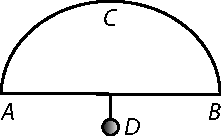
\includegraphics[width=0.26\textwidth]{gesamttex/edit_VIII-4/images/LH_37_03_065_d_065r.pdf}}%
  \vspace*{1.0em}
  \centerline{\lbrack\textit{Fig.\:1}\rbrack}%
\newpage%
\pstart%
\noindent%
\centering%
*     *     *
\pend%
\vspace{4.0em}%
\selectlanguage{latin}%
\frenchspacing%
\begin{ledgroup}%
\footnotesize%
\pstart%
\noindent%
\textls{Ausführliche Datierungsgründe:}%
\pagelabel{60198_dat}
Das im Träger der undatierten notizartigen Aufzeichnung N.\;\ref{60198} anzutreffende Wasserzeichen ist nach heutigem Wissensstand für die frühen Hannoveraner Jahre belegt, insbesondere für den Zeitraum vom Herbst 1677 bis zum Jahr 1682. %
Damals hat sich Leibniz intensiv mit Themen der Elastizitätstheorie und der Akustik befasst und in diesem Zusammenhang auch das mechanische Verhalten der gespannten Saiten untersucht, wie zahlreiche in \textit{LSB} VIII,\;3 veröffentlichte Texte zeigen.
Es ist somit wahrscheinlich, dass auch die Aufzeichnung N.\;\ref{60198} ungefähr im gleichen Zeitraum abgefasst wurde. %
\pend%
\pstart%
Der nicht ermittelte Briefrest auf der Rückseite des Trägers von N.\;\ref{60198} ermöglicht aber eine weitere Eingrenzung des Terminus post quem der Datierung.
Dort wird nämlich ein \textit{Meister Hans} erwähnt (vgl. die Beschreibung der Überlieferung, \refpassage{LH_37_03_065_065v_hans-1}{LH_37_03_065_065v_hans-2}), bei dem es sich aller Wahrscheinlichkeit nach um den Handwerker Hans Linsen\indexN{\textls{Linsen}, Hans (Meister Hans), gest. 1698} handelt, einen Müller und Zimmermann, der in der ersten Hälfte der 1680er Jahre in Leibnizens Auftrag Windmühlen im Harzgebiet\indexO{Harz} baute.
Der älteste sichere Beleg seiner Person im Leibniz-Briefwechsel ist Leibnizens Schreiben an Herzog Johann Friedrich wohl von Anfang August 1679 (vgl. \textit{LSB} I,\;2 N.\;157,\cite{02614} S.\;188.30; Linsens Brief an Leibniz vom 29.\;Dezember 1678\,/\,8.\;Januar 1679 ist unsicher datierbar, vgl. \textit{LSB} III,\;2 N.\;255,\cite{02613} S.\;595.26--28).
Daher ist unwahrscheinlich, dass der Briefrest auf dem Träger von N.\;\ref{60198} -- und somit auch die später abgefasste Aufzeichnung selbst -- vor dem Herbst 1679 entstand.
Da der Austausch zwischen Hans Linsen\indexN{\textls{Linsen}, Hans (Meister Hans), gest. 1698} und Leibniz in den folgenden Jahren häufiger wurde, ist es eher wahrscheinlich, dass die Aufzeichnung N.\;\ref{60198} später enstand.
\pend%
\pstart%
Für eine spätere Datierung spricht zudem, dass der in N.\;\ref{60198} festgehaltene Gedanke in ähnlicher Gestalt auch in der zwischen Sommer und November 1689 entstandenen ersten Fassung von Leibnizens \textit{Dynamica}, pars~II, sectio~I, prop.\;36 vorkommt: %
\textit{Nulla chorda vel catena gravis in alio situ quam verticali perfecte in rectam extendi potest vi mortua; potest viva} (\textit{CFP}~I, S.\;340.2--4~[A]; S.\;579.22--24~[B]; III, S.\;414.20--22~[C]).\cite{01354}
Eine Entstehung der Aufzeichnung N.\;\ref{60198} während der Italienreise\indexO{Italien} ist jedoch schon aufgrund des Papiers extrem unwahrscheinlich.
Ferner gilt es zu beachten, dass in N.\;\ref{60198} die im zitierten Text der \textit{Dynamica}\cite{01354} hervorgehobene Unterscheidung zwischen "toter" und "lebendiger" Kraft unberücksichtigt bleibt.
Dies plädiert für eine frühe Entstehung von N.\;\ref{60198}.
Es bietet sich demnach an, den Terminus ante quem der Datierung an den Belegzeitraum des Wasserzeichens anzulehnen, ohne die Möglichkeit ausschließen zu können, dass N.\;\ref{60198} etwas später im Laufe der 1680er Jahre angefertig wurde.
\pend%
\pstart%
Als Datierung der Aufzeichnung N.\;\ref{60198} ergibt sich insgesamt die Zeitspanne \textit{Herbst 1679 bis 1682}.
Eine frühere Datierung ist unwahrscheinlich.
Eine spätere Datierung ist nicht auszuschließen.
\pend%
\end{ledgroup}%
\selectlanguage{latin}%
\frenchspacing%
\newpage%
